\documentclass[../../../main.tex]{subfiles}

\begin{document}

\section{Homothety}

Homothety is a type of linear transformation that concerns dilation.
Although it is a projective transformation, we consider this as a
topic in Euclidean geometry. In this section, we are going to review
important topics and properties in homothety.

\begin{definition}{}{}
\textbf{Homothety} is a linear dilation of a point $A$ from a point
$P$ with factor $k$ such that $k\vec{AP} = \vec{A'P}$ where $A'$ is
the \textbf{image} of $A$.
\end{definition}

For a more visual explanation, consider the following diagrams that
are both homothetic to center $P$.

\begin{minipage}{0.48\textwidth}
\begin{figure}[H]
\centering
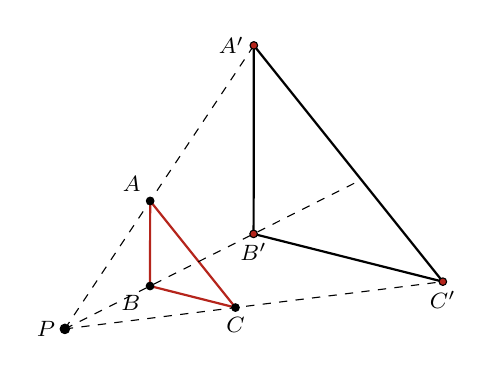
\begin{tikzpicture}[scale=0.6]
    \coordinate (P) at (0, 0);
    \coordinate (A) at (1.8054545454545454,2.708181818181818);
    \coordinate (B) at (1.8030484267241438,0.9075077811498734);
    \coordinate (C) at (3.610909090909091,0.45136363636363636);
    \coordinate (A') at (4,6);
    \coordinate (B') at (3.9946692233566123,2.0105912573310385);
    \coordinate (C') at (8,1);
    \coordinate (v1) at (6.273817034700317,3.157728706624606);

    \draw[thick,BrickRed] (A) -- (B) -- (C) -- cycle;
    \draw[thick] (A') -- (B') -- (C') -- cycle;

    \draw[thin,dashed] (P) -- (A');
    \draw[thin,dashed] (P) -- (v1);
    \draw[thin,dashed] (P) -- (C');

    \draw[fill=black] (A) circle (0.08)
        node[above left] {\footnotesize $A$};
    \draw[fill=black] (B) circle (0.08)
        node[below left] {\footnotesize $B$};
    \draw[fill=black] (C) circle (0.08)
        node[below] {\footnotesize $C$};
    \draw[fill=BrickRed] (A') circle (0.08)
        node[left] {\footnotesize $A'$};
    \draw[fill=BrickRed] (B') circle (0.08)
        node[below] {\footnotesize $B'$};
    \draw[fill=BrickRed] (C') circle (0.08)
        node[below] {\footnotesize $C'$};

    \draw[fill=black] (P) circle (0.1)
        node[left] {\footnotesize $P$};
\end{tikzpicture}
\end{figure}
\end{minipage}
\hfill
\begin{minipage}{0.48\textwidth}
\begin{figure}[H]
\centering
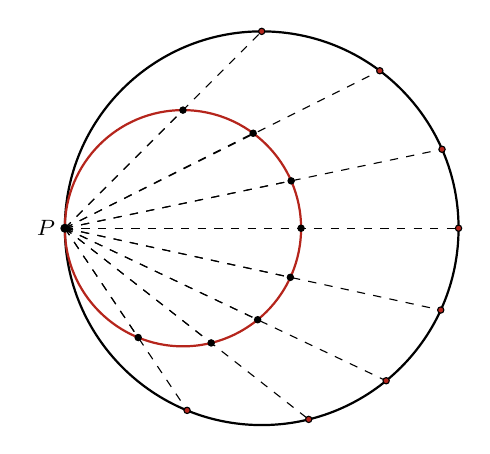
\begin{tikzpicture}[scale=0.5]
    \coordinate (P) at (-5,0);
    \coordinate (p11) at (0,5);
    \coordinate (p12) at (3,4);
    \coordinate (p13) at (4.5803775385576335,2.0050290781623876);
    \coordinate (p14) at (5,0);
    \coordinate (p15) at (4.547674363849642,-2.078138080201784);
    \coordinate (p16) at (3.1610407864167773,-3.87399292030969);
    \coordinate (p17) at (1.193521277317255,-4.855461559995197);
    \coordinate (p18) at (-1.8951266259437494,-4.626931496320111);
    \coordinate (p21) at (-2,3);
    \coordinate (p22) at (-0.21730574985800466,2.412882344937413);
    \coordinate (p23) at (0.7482265231345803,1.2030174468974324);
    \coordinate (p24) at (1,0);
    \coordinate (p25) at (0.7286046183097848,-1.2468828481210705);
    \coordinate (p26) at (-0.10337552814993366,-2.324395752185814);
    \coordinate (p27) at (-1.2838872336096472,-2.913276935997118);
    \coordinate (p28) at (-3.13707597556625,-2.7761588977920666);

    \draw[thick] (0, 0) circle (5);
    \draw[thick,BrickRed] (-2, 0) circle (3);

    \draw[thin,dashed] (P) -- (p11);
    \draw[thin,dashed] (P) -- (p12);
    \draw[thin,dashed] (P) -- (p13);
    \draw[thin,dashed] (P) -- (p14);
    \draw[thin,dashed] (P) -- (p15);
    \draw[thin,dashed] (P) -- (p16);
    \draw[thin,dashed] (P) -- (p17);
    \draw[thin,dashed] (P) -- (p18);
    \draw[thin,dashed] (P) -- (p21);
    \draw[thin,dashed] (P) -- (p22);
    \draw[thin,dashed] (P) -- (p23);
    \draw[thin,dashed] (P) -- (p24);
    \draw[thin,dashed] (P) -- (p25);
    \draw[thin,dashed] (P) -- (p26);
    \draw[thin,dashed] (P) -- (p27);
    \draw[thin,dashed] (P) -- (p28);

    \draw[fill=BrickRed] (p11) circle (0.08);
    \draw[fill=BrickRed] (p12) circle (0.08);
    \draw[fill=BrickRed] (p13) circle (0.08);
    \draw[fill=BrickRed] (p14) circle (0.08);
    \draw[fill=BrickRed] (p15) circle (0.08);
    \draw[fill=BrickRed] (p16) circle (0.08);
    \draw[fill=BrickRed] (p17) circle (0.08);
    \draw[fill=BrickRed] (p18) circle (0.08);
    \draw[fill=black] (p21) circle (0.08);
    \draw[fill=black] (p22) circle (0.08);
    \draw[fill=black] (p23) circle (0.08);
    \draw[fill=black] (p24) circle (0.08);
    \draw[fill=black] (p25) circle (0.08);
    \draw[fill=black] (p26) circle (0.08);
    \draw[fill=black] (p27) circle (0.08);
    \draw[fill=black] (p28) circle (0.08);

    \draw[fill=black] (P) circle (0.1)
        node[left] {\footnotesize $P$};
\end{tikzpicture}
\end{figure}
\end{minipage}

As you can see from the diagram above, the homothetic center,
a point, and its image are collinear. Also, a figure and its
image is also similar.

\begin{important}
This can come especially handy when we have to prove collinearity of
three points because if a triangle is an image of the other triangle,
then the homothetic center and the circumcenters of the triangles are
collinear.
\end{important}

I will skip the proof since it is quite straightforward using similar
triangles. Here is an example problem using the collinearity of the
three points.

\begin{problem}{2013 KMO Problem 1}{2013 KMO Problem 1}
Given a triangle $ABC$, let $P$ be a point on the side $BC$ and define
points $Q$ and $R$ as the intersections of the lines parallel to $AC$
and $AB$ that passes through $P$ with $AB$ and $AC$ respectively.
Let $O, O_1, O_2$ be the circumcenters of triangles $ABC, BPR, PCQ$
respectively. If $K \neq P$ is the intersection of the circumcircles
of $\triangle{BPR}$ and $\triangle{PCQ}$, show that $OO_1 = KO_2$.
\end{problem}
\begin{solution}
First, consider the following diagram.
\begin{figure}[H]
\centering
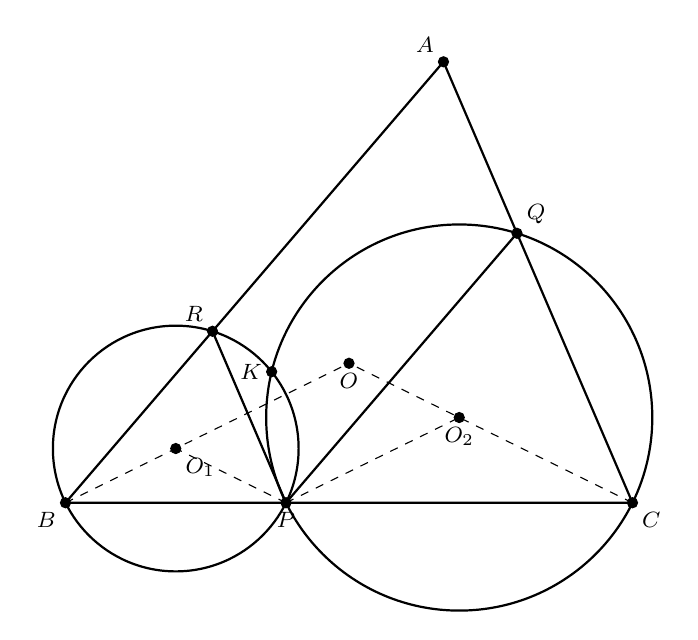
\begin{tikzpicture}[scale=0.8]
    \coordinate (A) at (6, 7);
    \coordinate (B) at (0, 0);
    \coordinate (C) at (9, 0);
    \coordinate (P) at (3.5,0);
    \coordinate (Q) at (7.166666666666667,4.277777777777778);
    \coordinate (R) at (2.3333333333333335,2.7222222222222223);
    \coordinate (K) at ((3.2725499718749713,2.0800671926917955);
    \coordinate (O) at (4.5,2.2142857142857144);
    \coordinate (O1) at (1.75,0.8611111111111112);
    \coordinate (O2) at (6.25,1.353174603174603);

    \draw[thick] (A) -- (B) -- (C) -- cycle;
    \draw[thick] (O1) circle (1.9503877423935512);
    \draw[thick] (O2) circle (3.0648950237612946);
    \draw[thick] (P) -- (R);
    \draw[thick] (P) -- (Q);

    \draw[thin, dashed] (B) -- (O);
    \draw[thin, dashed] (C) -- (O);
    \draw[thin, dashed] (P) -- (O1);
    \draw[thin, dashed] (P) -- (O2);

    \draw[fill=black] (A) circle (0.08)
        node[above left] {\footnotesize $A$};
    \draw[fill=black] (B) circle (0.08)
        node[below left] {\footnotesize $B$};
    \draw[fill=black] (C) circle (0.08)
        node[below right] {\footnotesize $C$};
    \draw[fill=black] (P) circle (0.08)
        node[below] {\footnotesize $P$};
    \draw[fill=black] (Q) circle (0.08)
        node[above right] {\footnotesize $Q$};
    \draw[fill=black] (R) circle (0.08)
        node[above left] {\footnotesize $R$};
    \draw[fill=black] (K) circle (0.08)
        node[left] {\footnotesize $K$};
    \draw[fill=black] (O) circle (0.08)
        node[below] {\footnotesize $O$};
    \draw[fill=black] (O1) circle (0.08)
        node[below right] {\footnotesize $O_1$};
    \draw[fill=black] (O2) circle (0.08)
        node[below] {\footnotesize $O_2$};
\end{tikzpicture}
\end{figure}

First, notice that because $KO_2 = PO_2$, it suffices to show that
quadrilateral $OO_1PO_2$ is a parallelogram. Let $\angle{BAC} =
\alpha$. Notice that $\angle{BO_1P} = \angle{PO_2C} = \angle{BOC} =
2\alpha$. Therefore, it suffices to show that $B, O_1, O$ and
$C, O_2, O$ are collinear. By construction, $\triangle{BRP}$
and $\triangle{BAC}$ and $\triangle{CQP}$ and $\triangle{CAB}$
are homothetic from $B$ and $C$ respectively. Thus, $OO_1 = KO_2$.
\end{solution}

With this basic idea in mind, let's discuss an important theorem.

\begin{theorem}{Monge's Theorem}{Monge's Theorem}
The pairwise external similitude centers of three distinct circles
are collinear.
\end{theorem}
\begin{proof}
First, consider the following diagram.
\begin{figure}[H]
\centering
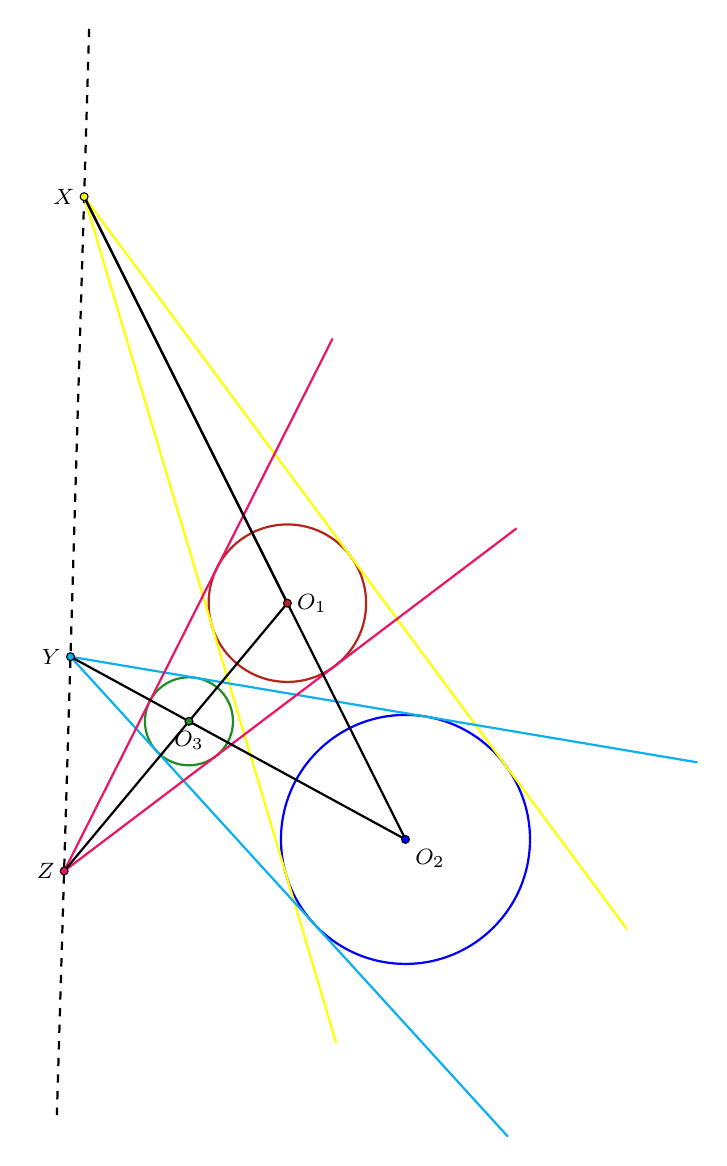
\begin{tikzpicture}[scale=0.25]
    \coordinate (O1) at (2,6);
    \coordinate (O2) at (8,-6);
    \coordinate (O3) at (-3,0);
    \coordinate (X) at (-8.324555320336787,26.649110640673555);
    \coordinate (Y) at (-9.016099767458295,3.28150896406816);
    \coordinate (Z) at (-9.338305413636002,-7.6059664963632);
    \coordinate (p1) at (4.478594673677544,-16.332420408971092);
    \coordinate (p2) at (19.249018279089587,-10.556561633949324);
    \coordinate (p3) at (13.203687791113277,-21.098898672680008);
    \coordinate (p4) at (22.831624730646023,-2.085863926492911);
    \coordinate (p5) at (4.30151507882518,19.451649497871916);
    \coordinate (p6) at (13.641555474983383,9.799845807662326);
    \coordinate (p7) at (-8.07,35.18);
    \coordinate (p8) at (-9.71,-20.01);

    \draw[thick,BrickRed] (O1) circle (4);
    \draw[thick,Blue] (O2) circle (6.324555320336759);
    \draw[thick,ForestGreen] (O3) circle (2.23606797749979);
    \draw[thick,dashed] (p7) -- (p8);
    \draw[thick,Yellow] (X) -- (p1);
    \draw[thick,Yellow] (X) -- (p2);
    \draw[thick,ProcessBlue] (Y) -- (p3);
    \draw[thick,ProcessBlue] (Y) -- (p4);
    \draw[thick,WildStrawberry] (Z) -- (p5);
    \draw[thick,WildStrawberry] (Z) -- (p6);
    \draw[thick] (O1) -- (X);
    \draw[thick] (O1) -- (Z);
    \draw[thick] (O2) -- (X);
    \draw[thick] (O2) -- (Y);

    \draw[fill=BrickRed] (O1) circle (0.2)
        node[right] {\footnotesize $O_1$};
    \draw[fill=Blue] (O2) circle (0.2)
        node[below right] {\footnotesize $O_2$};
    \draw[fill=ForestGreen] (O3) circle (0.2)
        node[below] {\footnotesize $O_3$};
    \draw[fill=Yellow] (X) circle (0.2)
        node[left] {\footnotesize $X$};
    \draw[fill=ProcessBlue] (Y) circle (0.2)
        node[left] {\footnotesize $Y$};
    \draw[fill=WildStrawberry] (Z) circle (0.2)
        node[left] {\footnotesize $Z$};
\end{tikzpicture}
\end{figure}

From the diagram above, it is evident that $X,Y,Z$ are collinear
if and only if Menelaus' Theorem holds for $\triangle{O_1O_2O_3}$.
In other words, it suffices to show that the following equation holds.
\[
\frac{O_2 X}{O_1 X} \cdot \frac{O_3 Y}{O_2 Y} \cdot
    \frac{O_1 Z}{O_3 Z}
= 1
\]
Note that $\frac{O_2 X}{O_1 X} = \frac{R_2}{R_1}$ by similar triangle.
Similarly, $\frac{O_3 Y}{O_2 Y} = \frac{R_3}{R_2}$ and
$\frac{O_1 Z}{O_3 Z} = \frac{R_1}{R_3}$. Because $\frac{R_2}{R_1}
\cdot \frac{R_3}{R_2} \cdot \frac{R_1}{R_3} = 1$, the theorem holds.
\end{proof}

Homothety in my opinion very popular and powerful tool because it
gives the best conditions like parallel sides and similarity.
This is it for this section, and we will discuss more on different
points and circles of a triangle in the next section.

\end{document}


